% Options for packages loaded elsewhere
% Options for packages loaded elsewhere
\PassOptionsToPackage{unicode}{hyperref}
\PassOptionsToPackage{hyphens}{url}
\PassOptionsToPackage{dvipsnames,svgnames,x11names}{xcolor}
%
\documentclass[
  letterpaper,
  DIV=11,
  numbers=noendperiod]{scrartcl}
\usepackage{xcolor}
\usepackage{amsmath,amssymb}
\setcounter{secnumdepth}{5}
\usepackage{iftex}
\ifPDFTeX
  \usepackage[T1]{fontenc}
  \usepackage[utf8]{inputenc}
  \usepackage{textcomp} % provide euro and other symbols
\else % if luatex or xetex
  \usepackage{unicode-math} % this also loads fontspec
  \defaultfontfeatures{Scale=MatchLowercase}
  \defaultfontfeatures[\rmfamily]{Ligatures=TeX,Scale=1}
\fi
\usepackage{lmodern}
\ifPDFTeX\else
  % xetex/luatex font selection
\fi
% Use upquote if available, for straight quotes in verbatim environments
\IfFileExists{upquote.sty}{\usepackage{upquote}}{}
\IfFileExists{microtype.sty}{% use microtype if available
  \usepackage[]{microtype}
  \UseMicrotypeSet[protrusion]{basicmath} % disable protrusion for tt fonts
}{}
\makeatletter
\@ifundefined{KOMAClassName}{% if non-KOMA class
  \IfFileExists{parskip.sty}{%
    \usepackage{parskip}
  }{% else
    \setlength{\parindent}{0pt}
    \setlength{\parskip}{6pt plus 2pt minus 1pt}}
}{% if KOMA class
  \KOMAoptions{parskip=half}}
\makeatother
% Make \paragraph and \subparagraph free-standing
\makeatletter
\ifx\paragraph\undefined\else
  \let\oldparagraph\paragraph
  \renewcommand{\paragraph}{
    \@ifstar
      \xxxParagraphStar
      \xxxParagraphNoStar
  }
  \newcommand{\xxxParagraphStar}[1]{\oldparagraph*{#1}\mbox{}}
  \newcommand{\xxxParagraphNoStar}[1]{\oldparagraph{#1}\mbox{}}
\fi
\ifx\subparagraph\undefined\else
  \let\oldsubparagraph\subparagraph
  \renewcommand{\subparagraph}{
    \@ifstar
      \xxxSubParagraphStar
      \xxxSubParagraphNoStar
  }
  \newcommand{\xxxSubParagraphStar}[1]{\oldsubparagraph*{#1}\mbox{}}
  \newcommand{\xxxSubParagraphNoStar}[1]{\oldsubparagraph{#1}\mbox{}}
\fi
\makeatother

\usepackage{color}
\usepackage{fancyvrb}
\newcommand{\VerbBar}{|}
\newcommand{\VERB}{\Verb[commandchars=\\\{\}]}
\DefineVerbatimEnvironment{Highlighting}{Verbatim}{commandchars=\\\{\}}
% Add ',fontsize=\small' for more characters per line
\usepackage{framed}
\definecolor{shadecolor}{RGB}{241,243,245}
\newenvironment{Shaded}{\begin{snugshade}}{\end{snugshade}}
\newcommand{\AlertTok}[1]{\textcolor[rgb]{0.68,0.00,0.00}{#1}}
\newcommand{\AnnotationTok}[1]{\textcolor[rgb]{0.37,0.37,0.37}{#1}}
\newcommand{\AttributeTok}[1]{\textcolor[rgb]{0.40,0.45,0.13}{#1}}
\newcommand{\BaseNTok}[1]{\textcolor[rgb]{0.68,0.00,0.00}{#1}}
\newcommand{\BuiltInTok}[1]{\textcolor[rgb]{0.00,0.23,0.31}{#1}}
\newcommand{\CharTok}[1]{\textcolor[rgb]{0.13,0.47,0.30}{#1}}
\newcommand{\CommentTok}[1]{\textcolor[rgb]{0.37,0.37,0.37}{#1}}
\newcommand{\CommentVarTok}[1]{\textcolor[rgb]{0.37,0.37,0.37}{\textit{#1}}}
\newcommand{\ConstantTok}[1]{\textcolor[rgb]{0.56,0.35,0.01}{#1}}
\newcommand{\ControlFlowTok}[1]{\textcolor[rgb]{0.00,0.23,0.31}{\textbf{#1}}}
\newcommand{\DataTypeTok}[1]{\textcolor[rgb]{0.68,0.00,0.00}{#1}}
\newcommand{\DecValTok}[1]{\textcolor[rgb]{0.68,0.00,0.00}{#1}}
\newcommand{\DocumentationTok}[1]{\textcolor[rgb]{0.37,0.37,0.37}{\textit{#1}}}
\newcommand{\ErrorTok}[1]{\textcolor[rgb]{0.68,0.00,0.00}{#1}}
\newcommand{\ExtensionTok}[1]{\textcolor[rgb]{0.00,0.23,0.31}{#1}}
\newcommand{\FloatTok}[1]{\textcolor[rgb]{0.68,0.00,0.00}{#1}}
\newcommand{\FunctionTok}[1]{\textcolor[rgb]{0.28,0.35,0.67}{#1}}
\newcommand{\ImportTok}[1]{\textcolor[rgb]{0.00,0.46,0.62}{#1}}
\newcommand{\InformationTok}[1]{\textcolor[rgb]{0.37,0.37,0.37}{#1}}
\newcommand{\KeywordTok}[1]{\textcolor[rgb]{0.00,0.23,0.31}{\textbf{#1}}}
\newcommand{\NormalTok}[1]{\textcolor[rgb]{0.00,0.23,0.31}{#1}}
\newcommand{\OperatorTok}[1]{\textcolor[rgb]{0.37,0.37,0.37}{#1}}
\newcommand{\OtherTok}[1]{\textcolor[rgb]{0.00,0.23,0.31}{#1}}
\newcommand{\PreprocessorTok}[1]{\textcolor[rgb]{0.68,0.00,0.00}{#1}}
\newcommand{\RegionMarkerTok}[1]{\textcolor[rgb]{0.00,0.23,0.31}{#1}}
\newcommand{\SpecialCharTok}[1]{\textcolor[rgb]{0.37,0.37,0.37}{#1}}
\newcommand{\SpecialStringTok}[1]{\textcolor[rgb]{0.13,0.47,0.30}{#1}}
\newcommand{\StringTok}[1]{\textcolor[rgb]{0.13,0.47,0.30}{#1}}
\newcommand{\VariableTok}[1]{\textcolor[rgb]{0.07,0.07,0.07}{#1}}
\newcommand{\VerbatimStringTok}[1]{\textcolor[rgb]{0.13,0.47,0.30}{#1}}
\newcommand{\WarningTok}[1]{\textcolor[rgb]{0.37,0.37,0.37}{\textit{#1}}}

\usepackage{longtable,booktabs,array}
\newcounter{none} % for unnumbered tables
\usepackage{calc} % for calculating minipage widths
% Correct order of tables after \paragraph or \subparagraph
\usepackage{etoolbox}
\makeatletter
\patchcmd\longtable{\par}{\if@noskipsec\mbox{}\fi\par}{}{}
\makeatother
% Allow footnotes in longtable head/foot
\IfFileExists{footnotehyper.sty}{\usepackage{footnotehyper}}{\usepackage{footnote}}
\makesavenoteenv{longtable}
\usepackage{graphicx}
\makeatletter
\newsavebox\pandoc@box
\newcommand*\pandocbounded[1]{% scales image to fit in text height/width
  \sbox\pandoc@box{#1}%
  \Gscale@div\@tempa{\textheight}{\dimexpr\ht\pandoc@box+\dp\pandoc@box\relax}%
  \Gscale@div\@tempb{\linewidth}{\wd\pandoc@box}%
  \ifdim\@tempb\p@<\@tempa\p@\let\@tempa\@tempb\fi% select the smaller of both
  \ifdim\@tempa\p@<\p@\scalebox{\@tempa}{\usebox\pandoc@box}%
  \else\usebox{\pandoc@box}%
  \fi%
}
% Set default figure placement to htbp
\def\fps@figure{htbp}
\makeatother





\setlength{\emergencystretch}{3em} % prevent overfull lines

\providecommand{\tightlist}{%
  \setlength{\itemsep}{0pt}\setlength{\parskip}{0pt}}



 


\KOMAoption{captions}{tableheading}
\makeatletter
\@ifpackageloaded{caption}{}{\usepackage{caption}}
\AtBeginDocument{%
\ifdefined\contentsname
  \renewcommand*\contentsname{Table of contents}
\else
  \newcommand\contentsname{Table of contents}
\fi
\ifdefined\listfigurename
  \renewcommand*\listfigurename{List of Figures}
\else
  \newcommand\listfigurename{List of Figures}
\fi
\ifdefined\listtablename
  \renewcommand*\listtablename{List of Tables}
\else
  \newcommand\listtablename{List of Tables}
\fi
\ifdefined\figurename
  \renewcommand*\figurename{Figure}
\else
  \newcommand\figurename{Figure}
\fi
\ifdefined\tablename
  \renewcommand*\tablename{Table}
\else
  \newcommand\tablename{Table}
\fi
}
\@ifpackageloaded{float}{}{\usepackage{float}}
\floatstyle{ruled}
\@ifundefined{c@chapter}{\newfloat{codelisting}{h}{lop}}{\newfloat{codelisting}{h}{lop}[chapter]}
\floatname{codelisting}{Listing}
\newcommand*\listoflistings{\listof{codelisting}{List of Listings}}
\makeatother
\makeatletter
\makeatother
\makeatletter
\@ifpackageloaded{caption}{}{\usepackage{caption}}
\@ifpackageloaded{subcaption}{}{\usepackage{subcaption}}
\makeatother
\usepackage{bookmark}
\IfFileExists{xurl.sty}{\usepackage{xurl}}{} % add URL line breaks if available
\urlstyle{same}
% fallback for those not using the hyperref driver hyperxmp:
\makeatletter
\@ifundefined{xmpquote}{\newcommand{\xmpquote}[1]{#1}}{}
\makeatother
\hypersetup{
  pdftitle={EDS223 - Homework Assignment 2},
  pdfauthor={Elyse Owen},
  colorlinks=true,
  linkcolor={blue},
  filecolor={Maroon},
  citecolor={Blue},
  urlcolor={Blue},
  pdfcreator={LaTeX via pandoc}}


\title{EDS223 - Homework Assignment 2}
\usepackage{etoolbox}
\makeatletter
\providecommand{\subtitle}[1]{% add subtitle to \maketitle
  \apptocmd{\@title}{\par {\large #1 \par}}{}{}
}
\makeatother
\subtitle{Effects of Historical Redlining Across Los Angeles County}
\author{Elyse Owen}
\date{2026-10-24}
\begin{document}
\maketitle

\renewcommand*\contentsname{Table of contents}
{
\setcounter{tocdepth}{3}
\tableofcontents
}

From the map titled `Los Angeles County by Historical Redlining
Neighbourhoods', various geographic trends in where historically
redlined zones. There are very few redlined zones towards the northern,
and especially northeastern areas, while there more redlined zones to
the central and southern areas of the county. Additionally, in only a
few instances do Grade A (green) neighbourhoods border Grade D (red)
neighbourhoods; typically Grade A neighbourhoods border Grade B (blue)
neighbourhoods, while Grade D neighbourhoods border Grade C (yellow)
neighbourhoods. Grade A neighbourhoods also appear to typically slightly
smaller geographically, while Grade D neighbourhoods appear to have more
geographical variance.

In the chart `Percent of Low Income Residents by HOLC Grade', it is
shown that the lowest percentage of low-income residents are in Grade A,
while the highest percentage is within Grade D. From this, the
historical legacy of redlined zones by the Home Owners' Loan Corporation
(HOLC) becomes more explicit - the neighbourhoods that were considered
less desirable for investment and less safe in the 1930s continue to be
disadvantage and have higher levels of poverty. This trend continues in
the chart `PM2.5 Levels by HOLC Grade', with Grade A neighbhourhoods
having the lowest levels of PM2.5, and Grade D neighbourhoods having the
highest levels of PM2.5. However, the variance across the neighbourhood
grades is much less significant than what can be seen with the
percentage of low income residents; a contributing factor toward this is
likely the overall poor air quality within Los Angeles county.

A change in the trends focusing on Grade A and Grade D occurs when
looking at the number of pedestrian accidents by HOLC grade, with Grade
C having the highest amount of accidents, followed by Grade B. Grade A
still has the lowest amount of pedestrian accidents, however, Grade D
has the secondest fewest number of accidents. A similiar trend is
reflected when looking at the number of bicycle accidents across the
HOLC grades. Without further data, it is not possible to full explain
the differences, however, some contributing factors could include the
types and sizes of roads within each neighbourhood grade, as well as the
accessibility of bike paths and sidewalks. An additonal consideration
would be to look at the amount of residents within each neighbourhood
grade who are walking or cycling places, as this may also contribute to
the variances across the neighbourhoods.

\section{Load libaries sf, tmap, tidyverse,
spData}\label{load-libaries-sf-tmap-tidyverse-spdata}

\begin{Shaded}
\begin{Highlighting}[]
\FunctionTok{library}\NormalTok{(sf)}
\end{Highlighting}
\end{Shaded}

\begin{verbatim}
Linking to GEOS 3.13.0, GDAL 3.8.5, PROJ 9.5.1; sf_use_s2() is TRUE
\end{verbatim}

\begin{Shaded}
\begin{Highlighting}[]
\FunctionTok{library}\NormalTok{(tmap)}
\end{Highlighting}
\end{Shaded}

\begin{verbatim}
Registered S3 method overwritten by 'stars':
  method                  from
  st_interpolate_aw.stars sf  
\end{verbatim}

\begin{Shaded}
\begin{Highlighting}[]
\FunctionTok{library}\NormalTok{(tidyverse)}
\end{Highlighting}
\end{Shaded}

\begin{verbatim}
-- Attaching core tidyverse packages ------------------------ tidyverse 2.0.0 --
v dplyr     1.2.1     v readr     2.2.0
v forcats   1.0.1     v stringr   1.6.0
v ggplot2   4.0.3     v tibble    3.3.1
v lubridate 1.9.5     v tidyr     1.3.2
v purrr     1.2.2     
\end{verbatim}

\begin{verbatim}
-- Conflicts ------------------------------------------ tidyverse_conflicts() --
x dplyr::filter() masks stats::filter()
x dplyr::lag()    masks stats::lag()
i Use the conflicted package (<http://conflicted.r-lib.org/>) to force all conflicts to become errors
\end{verbatim}

\begin{Shaded}
\begin{Highlighting}[]
\FunctionTok{library}\NormalTok{(stars)}
\end{Highlighting}
\end{Shaded}

\begin{verbatim}
Loading required package: abind
\end{verbatim}

\begin{Shaded}
\begin{Highlighting}[]
\FunctionTok{library}\NormalTok{(here)}
\end{Highlighting}
\end{Shaded}

\begin{verbatim}
here() starts at /Users/elyseowen/Desktop/School/UCSB/MEDS/eds223/EDS223-HW2
\end{verbatim}

\begin{Shaded}
\begin{Highlighting}[]
\FunctionTok{library}\NormalTok{(gt)}
\end{Highlighting}
\end{Shaded}

\begin{verbatim}

Attaching package: 'gt'

The following object is masked from 'package:tmap':

    metro
\end{verbatim}

\begin{Shaded}
\begin{Highlighting}[]
\FunctionTok{library}\NormalTok{(dplyr)}
\end{Highlighting}
\end{Shaded}

\section{Load the data}\label{load-the-data}

\begin{Shaded}
\begin{Highlighting}[]
\NormalTok{ej\_screen }\OtherTok{\textless{}{-}} \FunctionTok{st\_read}\NormalTok{(}\FunctionTok{here}\NormalTok{(}\StringTok{"data"}\NormalTok{, }\StringTok{"ejscreen"}\NormalTok{, }\StringTok{"EJSCREEN\_2023\_BG\_StatePct\_with\_AS\_CNMI\_GU\_VI.gdb"}\NormalTok{))}
\end{Highlighting}
\end{Shaded}

\begin{verbatim}
Reading layer `EJSCREEN_StatePctiles_with_AS_CNMI_GU_VI' from data source 
  `/Users/elyseowen/Desktop/School/UCSB/MEDS/eds223/EDS223-HW2/data/ejscreen/EJSCREEN_2023_BG_StatePct_with_AS_CNMI_GU_VI.gdb' 
  using driver `OpenFileGDB'
Simple feature collection with 243021 features and 223 fields
Geometry type: MULTIPOLYGON
Dimension:     XY
Bounding box:  xmin: -19951910 ymin: -1617130 xmax: 16259830 ymax: 11554350
Projected CRS: WGS 84 / Pseudo-Mercator
\end{verbatim}

\begin{Shaded}
\begin{Highlighting}[]
\NormalTok{inequality }\OtherTok{\textless{}{-}} \FunctionTok{st\_read}\NormalTok{(}\FunctionTok{here}\NormalTok{(}\StringTok{"data"}\NormalTok{, }\StringTok{"mapping{-}inequality"}\NormalTok{, }\StringTok{"mapping{-}inequality{-}los{-}angeles.json"}\NormalTok{))}
\end{Highlighting}
\end{Shaded}

\begin{verbatim}
Reading layer `mapping-inequality-los-angeles' from data source 
  `/Users/elyseowen/Desktop/School/UCSB/MEDS/eds223/EDS223-HW2/data/mapping-inequality/mapping-inequality-los-angeles.json' 
  using driver `GeoJSON'
Simple feature collection with 417 features and 14 fields
Geometry type: MULTIPOLYGON
Dimension:     XY
Bounding box:  xmin: -118.6104 ymin: 33.70563 xmax: -117.7028 ymax: 34.30388
Geodetic CRS:  WGS 84
\end{verbatim}

\begin{Shaded}
\begin{Highlighting}[]
\NormalTok{crashes }\OtherTok{\textless{}{-}} \FunctionTok{read\_csv}\NormalTok{(}\StringTok{\textquotesingle{}data/SWITRS\_LA/Crashes.csv\textquotesingle{}}\NormalTok{)}
\end{Highlighting}
\end{Shaded}

\begin{verbatim}
Rows: 251100 Columns: 80
-- Column specification --------------------------------------------------------
Delimiter: ","
chr  (45): COLLISION_TIME, OFFICER_ID, REPORTING_DISTRICT, CHP_BEAT_TYPE, CI...
dbl  (33): CASE_ID, ACCIDENT_YEAR, JURIS, DAY_OF_WEEK, CHP_SHIFT, POPULATION...
date  (2): PROC_DATE, COLLISION_DATE

i Use `spec()` to retrieve the full column specification for this data.
i Specify the column types or set `show_col_types = FALSE` to quiet this message.
\end{verbatim}

\section{Filter to Los Angeles
County}\label{filter-to-los-angeles-county}

\begin{Shaded}
\begin{Highlighting}[]
\NormalTok{california }\OtherTok{\textless{}{-}}\NormalTok{ ej\_screen }\SpecialCharTok{\%\textgreater{}\%}
\NormalTok{  dplyr}\SpecialCharTok{::}\FunctionTok{filter}\NormalTok{(ST\_ABBREV }\SpecialCharTok{==} \StringTok{"CA"}\NormalTok{)}

\NormalTok{los\_angeles}\OtherTok{\textless{}{-}}\NormalTok{ california }\SpecialCharTok{\%\textgreater{}\%}
\NormalTok{  dplyr}\SpecialCharTok{::}\FunctionTok{filter}\NormalTok{(CNTY\_NAME }\SpecialCharTok{\%in\%} \FunctionTok{c}\NormalTok{(}\StringTok{"Los Angeles County"}\NormalTok{))}
\end{Highlighting}
\end{Shaded}

\section{Match the CRS}\label{match-the-crs}

\begin{Shaded}
\begin{Highlighting}[]
\FunctionTok{st\_crs}\NormalTok{(los\_angeles)}
\end{Highlighting}
\end{Shaded}

\begin{verbatim}
Coordinate Reference System:
  User input: WGS 84 / Pseudo-Mercator 
  wkt:
PROJCRS["WGS 84 / Pseudo-Mercator",
    BASEGEOGCRS["WGS 84",
        ENSEMBLE["World Geodetic System 1984 ensemble",
            MEMBER["World Geodetic System 1984 (Transit)"],
            MEMBER["World Geodetic System 1984 (G730)"],
            MEMBER["World Geodetic System 1984 (G873)"],
            MEMBER["World Geodetic System 1984 (G1150)"],
            MEMBER["World Geodetic System 1984 (G1674)"],
            MEMBER["World Geodetic System 1984 (G1762)"],
            MEMBER["World Geodetic System 1984 (G2139)"],
            MEMBER["World Geodetic System 1984 (G2296)"],
            ELLIPSOID["WGS 84",6378137,298.257223563,
                LENGTHUNIT["metre",1]],
            ENSEMBLEACCURACY[2.0]],
        PRIMEM["Greenwich",0,
            ANGLEUNIT["degree",0.0174532925199433]],
        ID["EPSG",4326]],
    CONVERSION["Popular Visualisation Pseudo-Mercator",
        METHOD["Popular Visualisation Pseudo Mercator",
            ID["EPSG",1024]],
        PARAMETER["Latitude of natural origin",0,
            ANGLEUNIT["degree",0.0174532925199433],
            ID["EPSG",8801]],
        PARAMETER["Longitude of natural origin",0,
            ANGLEUNIT["degree",0.0174532925199433],
            ID["EPSG",8802]],
        PARAMETER["False easting",0,
            LENGTHUNIT["metre",1],
            ID["EPSG",8806]],
        PARAMETER["False northing",0,
            LENGTHUNIT["metre",1],
            ID["EPSG",8807]]],
    CS[Cartesian,2],
        AXIS["easting (X)",east,
            ORDER[1],
            LENGTHUNIT["metre",1]],
        AXIS["northing (Y)",north,
            ORDER[2],
            LENGTHUNIT["metre",1]],
    USAGE[
        SCOPE["Web mapping and visualisation."],
        AREA["World between 85.06°S and 85.06°N."],
        BBOX[-85.06,-180,85.06,180]],
    ID["EPSG",3857]]
\end{verbatim}

\begin{Shaded}
\begin{Highlighting}[]
\FunctionTok{st\_crs}\NormalTok{(inequality)}
\end{Highlighting}
\end{Shaded}

\begin{verbatim}
Coordinate Reference System:
  User input: WGS 84 
  wkt:
GEOGCRS["WGS 84",
    DATUM["World Geodetic System 1984",
        ELLIPSOID["WGS 84",6378137,298.257223563,
            LENGTHUNIT["metre",1]]],
    PRIMEM["Greenwich",0,
        ANGLEUNIT["degree",0.0174532925199433]],
    CS[ellipsoidal,2],
        AXIS["geodetic latitude (Lat)",north,
            ORDER[1],
            ANGLEUNIT["degree",0.0174532925199433]],
        AXIS["geodetic longitude (Lon)",east,
            ORDER[2],
            ANGLEUNIT["degree",0.0174532925199433]],
    ID["EPSG",4326]]
\end{verbatim}

\begin{Shaded}
\begin{Highlighting}[]
\FunctionTok{st\_crs}\NormalTok{(los\_angeles) }\SpecialCharTok{==} \FunctionTok{st\_crs}\NormalTok{(inequality)}
\end{Highlighting}
\end{Shaded}

\begin{verbatim}
[1] FALSE
\end{verbatim}

\begin{Shaded}
\begin{Highlighting}[]
\NormalTok{la\_transform }\OtherTok{\textless{}{-}} \FunctionTok{st\_transform}\NormalTok{(los\_angeles, }\AttributeTok{crs =} \FunctionTok{st\_crs}\NormalTok{(inequality))}
\ControlFlowTok{if}\NormalTok{(}\FunctionTok{st\_crs}\NormalTok{(la\_transform) }\SpecialCharTok{==} \FunctionTok{st\_crs}\NormalTok{(inequality))\{}
  \FunctionTok{print}\NormalTok{(}\StringTok{"it\textquotesingle{}s a match!"}\NormalTok{)}
\NormalTok{\} }\ControlFlowTok{else}\NormalTok{ \{}
  \FunctionTok{print}\NormalTok{(}\StringTok{"still not a match"}\NormalTok{)}
\NormalTok{\}}
\end{Highlighting}
\end{Shaded}

\begin{verbatim}
[1] "it's a match!"
\end{verbatim}

\section{Join the dataframes, drop the
geometry}\label{join-the-dataframes-drop-the-geometry}

\begin{Shaded}
\begin{Highlighting}[]
\NormalTok{la\_transform }\OtherTok{\textless{}{-}} \FunctionTok{st\_make\_valid}\NormalTok{(la\_transform)}
\NormalTok{inequality }\OtherTok{\textless{}{-}} \FunctionTok{st\_make\_valid}\NormalTok{(inequality)}
\NormalTok{la\_inequality }\OtherTok{\textless{}{-}} \FunctionTok{st\_join}\NormalTok{(la\_transform, inequality, }\AttributeTok{left =} \ConstantTok{FALSE}\NormalTok{)}
\NormalTok{la\_inequality }\OtherTok{\textless{}{-}} \FunctionTok{st\_drop\_geometry}\NormalTok{(la\_inequality)}
\end{Highlighting}
\end{Shaded}

\section{Create a colour palette}\label{create-a-colour-palette}

\begin{Shaded}
\begin{Highlighting}[]
\NormalTok{grade\_colors\_transparent }\OtherTok{\textless{}{-}} \FunctionTok{c}\NormalTok{(}\StringTok{"A"} \OtherTok{=} \StringTok{"\#0855016f"}\NormalTok{, }\StringTok{"B"} \OtherTok{=} \StringTok{"\#00588b5e"}\NormalTok{, }\StringTok{"C"} \OtherTok{=} \StringTok{"\#bfb90360"}\NormalTok{, }\StringTok{"D"} \OtherTok{=}\StringTok{"\#c40017c2"}\NormalTok{)}

\NormalTok{grade\_colors}\OtherTok{\textless{}{-}} \FunctionTok{c}\NormalTok{(}\StringTok{"A"} \OtherTok{=} \StringTok{"\#76A865"}\NormalTok{, }\StringTok{"B"} \OtherTok{=} \StringTok{"\#7CB5BD"}\NormalTok{, }\StringTok{"C"} \OtherTok{=} \StringTok{"\#FFFF00"}\NormalTok{, }\StringTok{"D"} \OtherTok{=}\StringTok{"\#e30c25"}\NormalTok{)}
\end{Highlighting}
\end{Shaded}

\subsection{Map of historical
redlining}\label{map-of-historical-redlining}

\begin{Shaded}
\begin{Highlighting}[]
\FunctionTok{tm\_basemap}\NormalTok{(}\StringTok{\textquotesingle{}OpenStreetMap.HOT\textquotesingle{}}\NormalTok{, }\AttributeTok{alpha =} \FloatTok{0.7}\NormalTok{)}\SpecialCharTok{+}
    \FunctionTok{tm\_shape}\NormalTok{(inequality, }\AttributeTok{alpha =} \FloatTok{0.7}\NormalTok{)}\SpecialCharTok{+}
    \FunctionTok{tm\_polygons}\NormalTok{(}\AttributeTok{fill =} \StringTok{\textquotesingle{}grade\textquotesingle{}}\NormalTok{, }
    \AttributeTok{fill.scale =} \FunctionTok{tm\_scale}\NormalTok{(}\AttributeTok{values =}\NormalTok{ grade\_colors\_transparent))}\SpecialCharTok{+}
    \FunctionTok{tm\_title}\NormalTok{(}\StringTok{"Los Angeles County by Historical Redlining Neighbourhoods"}\NormalTok{)}\SpecialCharTok{+}
\FunctionTok{tm\_compass}\NormalTok{(}\AttributeTok{position =} \FunctionTok{c}\NormalTok{(}\StringTok{\textquotesingle{}right\textquotesingle{}}\NormalTok{, }\StringTok{\textquotesingle{}top\textquotesingle{}}\NormalTok{))}\SpecialCharTok{+}
\FunctionTok{tm\_scalebar}\NormalTok{()}
\end{Highlighting}
\end{Shaded}

\begin{verbatim}
[plot mode] fit legend/component: Some legend items or map compoments do not
fit well, and are therefore rescaled.
i Set the tmap option `component.autoscale = FALSE` to disable rescaling.
\end{verbatim}

\pandocbounded{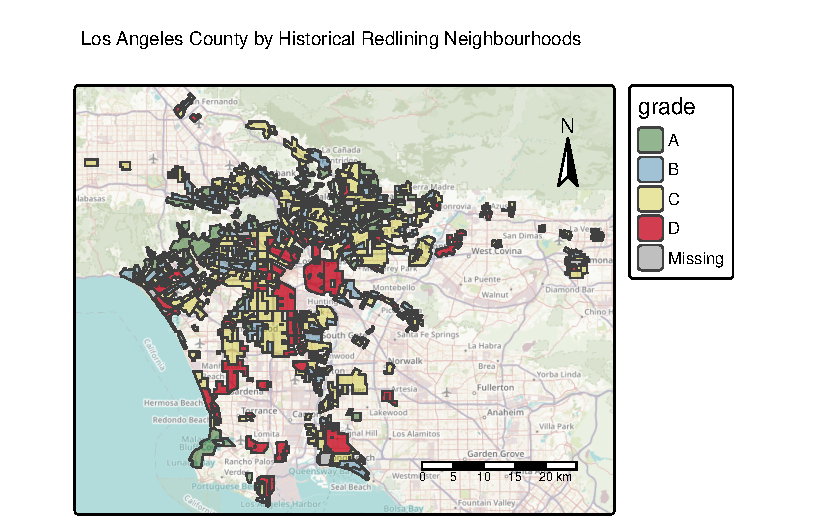
\includegraphics[keepaspectratio]{ejscreen_inequality_files/figure-pdf/unnamed-chunk-7-1.pdf}}

\section{Calculate percentage within each HOLC
grade}\label{calculate-percentage-within-each-holc-grade}

\begin{Shaded}
\begin{Highlighting}[]
\NormalTok{la\_inequality\_percent }\OtherTok{\textless{}{-}}\NormalTok{ la\_inequality }\SpecialCharTok{|\textgreater{}} 
  \FunctionTok{mutate}\NormalTok{(}
    \AttributeTok{grade =} \FunctionTok{ifelse}\NormalTok{(}\FunctionTok{is.na}\NormalTok{(grade), }\StringTok{\textquotesingle{}No Grade\textquotesingle{}}\NormalTok{, grade)) }\SpecialCharTok{|\textgreater{}} 
      \FunctionTok{count}\NormalTok{(grade) }\SpecialCharTok{|\textgreater{}} 
      \FunctionTok{mutate}\NormalTok{(}\AttributeTok{percent =}\NormalTok{ (n}\SpecialCharTok{/}\FunctionTok{sum}\NormalTok{(n))}\SpecialCharTok{*}\DecValTok{100}\NormalTok{)}
\end{Highlighting}
\end{Shaded}

\section{Create table of percentage of population within each HOLC
grade}\label{create-table-of-percentage-of-population-within-each-holc-grade}

\begin{Shaded}
\begin{Highlighting}[]
\NormalTok{redlining }\OtherTok{\textless{}{-}} \FunctionTok{data.frame}\NormalTok{(}
  \AttributeTok{Grade =} \FunctionTok{c}\NormalTok{(}\StringTok{"A"}\NormalTok{, }\StringTok{"B"}\NormalTok{, }\StringTok{"C"}\NormalTok{, }\StringTok{"D"}\NormalTok{, }\StringTok{"No Grade"}\NormalTok{),}
  \AttributeTok{Percent =} \FunctionTok{c}\NormalTok{(}\FloatTok{7.03}\NormalTok{, }\FloatTok{19.40}\NormalTok{, }\FloatTok{47.87}\NormalTok{, }\FloatTok{21.07}\NormalTok{, }\FloatTok{4.63}\NormalTok{)}
\NormalTok{)}
\end{Highlighting}
\end{Shaded}

\section{Create data frames of mean percent of population classified as
low income, mean PM2.5 concentration levels, by HOLC
grade}\label{create-data-frames-of-mean-percent-of-population-classified-as-low-income-mean-pm2.5-concentration-levels-by-holc-grade}

\begin{Shaded}
\begin{Highlighting}[]
\NormalTok{low\_income }\OtherTok{\textless{}{-}}\NormalTok{ la\_inequality }\SpecialCharTok{|\textgreater{}} 
  \FunctionTok{summarise}\NormalTok{(}\AttributeTok{low\_income\_mean =} \FunctionTok{mean}\NormalTok{(LOWINCPCT), }\AttributeTok{.by =} \StringTok{\textquotesingle{}grade\textquotesingle{}}\NormalTok{)}

\NormalTok{pm\_25 }\OtherTok{\textless{}{-}}\NormalTok{ la\_inequality }\SpecialCharTok{|\textgreater{}} 
  \FunctionTok{summarise}\NormalTok{(}\AttributeTok{mean\_pm\_25 =} \FunctionTok{mean}\NormalTok{(PM25), }\AttributeTok{.by =} \StringTok{\textquotesingle{}grade\textquotesingle{}}\NormalTok{)}
\end{Highlighting}
\end{Shaded}

\section{Visualise percentage of low income population, mean PM2.5
concentrations by HOLC
grade}\label{visualise-percentage-of-low-income-population-mean-pm2.5-concentrations-by-holc-grade}

\begin{Shaded}
\begin{Highlighting}[]
\FunctionTok{ggplot}\NormalTok{(}\AttributeTok{data =}\NormalTok{ low\_income, }\FunctionTok{aes}\NormalTok{(}\AttributeTok{fill =}\NormalTok{ grade)) }\SpecialCharTok{+}
  \FunctionTok{geom\_col}\NormalTok{(}\AttributeTok{mapping =} \FunctionTok{aes}\NormalTok{(}\AttributeTok{x =}\NormalTok{ grade, }\AttributeTok{y =}\NormalTok{ low\_income\_mean))}\SpecialCharTok{+}
  \FunctionTok{labs}\NormalTok{(}\AttributeTok{x =} \StringTok{\textquotesingle{}HOLC Grade\textquotesingle{}}\NormalTok{, }\AttributeTok{y =} \StringTok{\textquotesingle{}Percent Low Income\textquotesingle{}}\NormalTok{, }\AttributeTok{title =} \StringTok{\textquotesingle{}Percent of Low Income Residents by HOLC Grade\textquotesingle{}}\NormalTok{)}\SpecialCharTok{+}
  \FunctionTok{scale\_fill\_manual}\NormalTok{(}\AttributeTok{values =}\NormalTok{ grade\_colors, }\AttributeTok{name =} \StringTok{"Grade"}\NormalTok{)}
\end{Highlighting}
\end{Shaded}

\pandocbounded{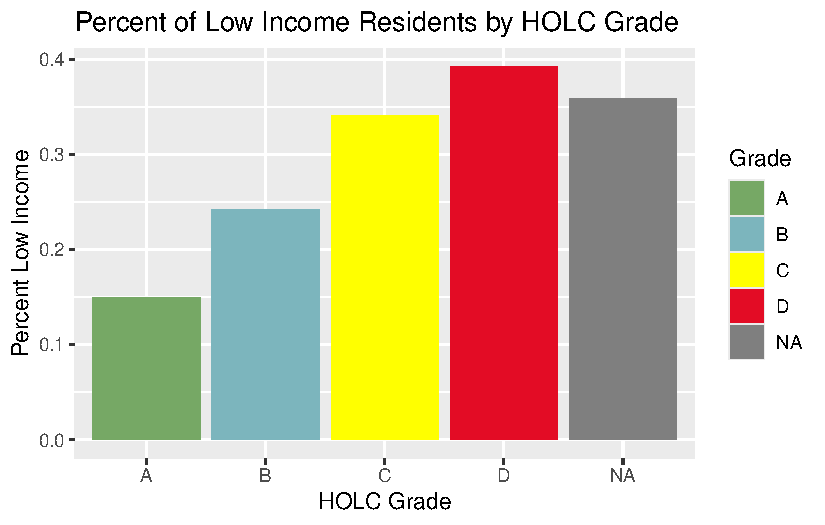
\includegraphics[keepaspectratio]{ejscreen_inequality_files/figure-pdf/unnamed-chunk-11-1.pdf}}

\begin{Shaded}
\begin{Highlighting}[]
\FunctionTok{ggplot}\NormalTok{(}\AttributeTok{data =}\NormalTok{ pm\_25, }\FunctionTok{aes}\NormalTok{(}\AttributeTok{fill =}\NormalTok{ grade)) }\SpecialCharTok{+}
  \FunctionTok{geom\_col}\NormalTok{(}\AttributeTok{mapping =} \FunctionTok{aes}\NormalTok{(}\AttributeTok{x =}\NormalTok{ grade, }\AttributeTok{y =}\NormalTok{ mean\_pm\_25))}\SpecialCharTok{+}
  \FunctionTok{labs}\NormalTok{(}\AttributeTok{x =} \StringTok{\textquotesingle{}HOLC Grade\textquotesingle{}}\NormalTok{, }\AttributeTok{y =} \StringTok{\textquotesingle{}PM2.5\textquotesingle{}}\NormalTok{, }\AttributeTok{title =} \StringTok{\textquotesingle{}PM2.5 Levels by HOLC Grade\textquotesingle{}}\NormalTok{)}\SpecialCharTok{+}
  \FunctionTok{scale\_fill\_manual}\NormalTok{(}\AttributeTok{values =}\NormalTok{ grade\_colors, }\AttributeTok{name =} \StringTok{"Grade"}\NormalTok{)}
\end{Highlighting}
\end{Shaded}

\pandocbounded{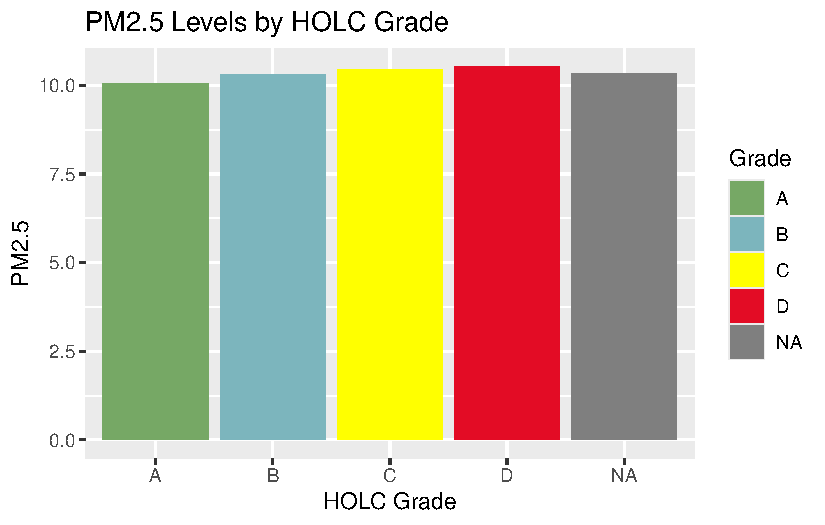
\includegraphics[keepaspectratio]{ejscreen_inequality_files/figure-pdf/unnamed-chunk-11-2.pdf}}

\section{Match CRS, join SWITRS data to HOLC data, drop
geometry}\label{match-crs-join-switrs-data-to-holc-data-drop-geometry}

\begin{Shaded}
\begin{Highlighting}[]
\NormalTok{crashes }\OtherTok{\textless{}{-}}\NormalTok{ crashes }\SpecialCharTok{|\textgreater{}} \FunctionTok{filter}\NormalTok{(}\SpecialCharTok{!}\FunctionTok{is.na}\NormalTok{(LATITUDE))}
\NormalTok{spatial\_crashes }\OtherTok{\textless{}{-}} \FunctionTok{st\_as\_sf}\NormalTok{(crashes, }\AttributeTok{coords =} \FunctionTok{c}\NormalTok{(}\StringTok{"LATITUDE"}\NormalTok{, }\StringTok{"LONGITUDE"}\NormalTok{), }\AttributeTok{crs =} \DecValTok{4326}\NormalTok{)}
\FunctionTok{st\_crs}\NormalTok{(inequality)}
\end{Highlighting}
\end{Shaded}

\begin{verbatim}
Coordinate Reference System:
  User input: WGS 84 
  wkt:
GEOGCRS["WGS 84",
    DATUM["World Geodetic System 1984",
        ELLIPSOID["WGS 84",6378137,298.257223563,
            LENGTHUNIT["metre",1]]],
    PRIMEM["Greenwich",0,
        ANGLEUNIT["degree",0.0174532925199433]],
    CS[ellipsoidal,2],
        AXIS["geodetic latitude (Lat)",north,
            ORDER[1],
            ANGLEUNIT["degree",0.0174532925199433]],
        AXIS["geodetic longitude (Lon)",east,
            ORDER[2],
            ANGLEUNIT["degree",0.0174532925199433]],
    ID["EPSG",4326]]
\end{verbatim}

\begin{Shaded}
\begin{Highlighting}[]
\FunctionTok{st\_crs}\NormalTok{(spatial\_crashes)}
\end{Highlighting}
\end{Shaded}

\begin{verbatim}
Coordinate Reference System:
  User input: EPSG:4326 
  wkt:
GEOGCRS["WGS 84",
    ENSEMBLE["World Geodetic System 1984 ensemble",
        MEMBER["World Geodetic System 1984 (Transit)"],
        MEMBER["World Geodetic System 1984 (G730)"],
        MEMBER["World Geodetic System 1984 (G873)"],
        MEMBER["World Geodetic System 1984 (G1150)"],
        MEMBER["World Geodetic System 1984 (G1674)"],
        MEMBER["World Geodetic System 1984 (G1762)"],
        MEMBER["World Geodetic System 1984 (G2139)"],
        MEMBER["World Geodetic System 1984 (G2296)"],
        ELLIPSOID["WGS 84",6378137,298.257223563,
            LENGTHUNIT["metre",1]],
        ENSEMBLEACCURACY[2.0]],
    PRIMEM["Greenwich",0,
        ANGLEUNIT["degree",0.0174532925199433]],
    CS[ellipsoidal,2],
        AXIS["geodetic latitude (Lat)",north,
            ORDER[1],
            ANGLEUNIT["degree",0.0174532925199433]],
        AXIS["geodetic longitude (Lon)",east,
            ORDER[2],
            ANGLEUNIT["degree",0.0174532925199433]],
    USAGE[
        SCOPE["Horizontal component of 3D system."],
        AREA["World."],
        BBOX[-90,-180,90,180]],
    ID["EPSG",4326]]
\end{verbatim}

\begin{Shaded}
\begin{Highlighting}[]
\NormalTok{bike\_ped\_crashes }\OtherTok{\textless{}{-}}\NormalTok{ spatial\_crashes }\SpecialCharTok{|\textgreater{}} 
  \FunctionTok{select}\NormalTok{(PEDESTRIAN\_ACCIDENT, BICYCLE\_ACCIDENT, POINT\_X, POINT\_Y)}

\ControlFlowTok{if}\NormalTok{(}\FunctionTok{st\_crs}\NormalTok{(bike\_ped\_crashes) }\SpecialCharTok{==} \FunctionTok{st\_crs}\NormalTok{(inequality))\{}
  \FunctionTok{print}\NormalTok{(}\StringTok{"it\textquotesingle{}s a match!"}\NormalTok{)}
\NormalTok{\} }\ControlFlowTok{else}\NormalTok{ \{}
  \FunctionTok{print}\NormalTok{(}\StringTok{"still not a match"}\NormalTok{)}
\NormalTok{\}}
\end{Highlighting}
\end{Shaded}

\begin{verbatim}
[1] "it's a match!"
\end{verbatim}

\begin{Shaded}
\begin{Highlighting}[]
\NormalTok{HOLC\_bike\_peds }\OtherTok{\textless{}{-}} \FunctionTok{st\_join}\NormalTok{(inequality, bike\_ped\_crashes)}
\end{Highlighting}
\end{Shaded}

\begin{verbatim}
Warning in st_is_longlat(x): bounding box has potentially an invalid value
range for longlat data
\end{verbatim}

\begin{Shaded}
\begin{Highlighting}[]
\NormalTok{HOLC\_bike\_peds }\OtherTok{\textless{}{-}} \FunctionTok{st\_drop\_geometry}\NormalTok{(HOLC\_bike\_peds)}
\end{Highlighting}
\end{Shaded}

\section{Visualise bicycle, pedestrian accidents by HOLC
grade}\label{visualise-bicycle-pedestrian-accidents-by-holc-grade}

\begin{Shaded}
\begin{Highlighting}[]
\FunctionTok{ggplot}\NormalTok{(}\AttributeTok{data =}\NormalTok{ HOLC\_bike\_peds, }\FunctionTok{aes}\NormalTok{(}\AttributeTok{fill =}\NormalTok{ grade)) }\SpecialCharTok{+}
  \FunctionTok{geom\_col}\NormalTok{(}\AttributeTok{mapping =} \FunctionTok{aes}\NormalTok{(}\AttributeTok{x =}\NormalTok{ grade, }\AttributeTok{y =}\NormalTok{ PEDESTRIAN\_ACCIDENT))}\SpecialCharTok{+}
  \FunctionTok{labs}\NormalTok{(}\AttributeTok{x =} \StringTok{\textquotesingle{}HOLC Grade\textquotesingle{}}\NormalTok{, }\AttributeTok{y =} \StringTok{\textquotesingle{}Number of Pedestrian Accidents\textquotesingle{}}\NormalTok{, }\AttributeTok{title =} \StringTok{\textquotesingle{}Number of Pedistrian Accidents by HOLC Grade\textquotesingle{}}\NormalTok{)}\SpecialCharTok{+}
  \FunctionTok{scale\_fill\_manual}\NormalTok{(}\AttributeTok{values =}\NormalTok{ grade\_colors, }\AttributeTok{name =} \StringTok{"Grade"}\NormalTok{)}
\end{Highlighting}
\end{Shaded}

\pandocbounded{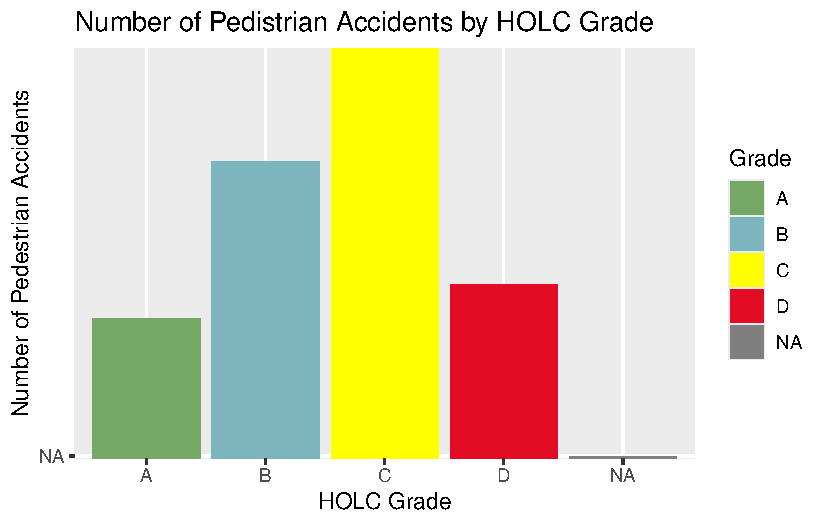
\includegraphics[keepaspectratio]{ejscreen_inequality_files/figure-pdf/unnamed-chunk-13-1.pdf}}

\begin{Shaded}
\begin{Highlighting}[]
\FunctionTok{ggplot}\NormalTok{(}\AttributeTok{data =}\NormalTok{ HOLC\_bike\_peds, }\FunctionTok{aes}\NormalTok{(}\AttributeTok{fill =}\NormalTok{ grade)) }\SpecialCharTok{+}
  \FunctionTok{geom\_col}\NormalTok{(}\AttributeTok{mapping =} \FunctionTok{aes}\NormalTok{(}\AttributeTok{x =}\NormalTok{ grade, }\AttributeTok{y =}\NormalTok{ BICYCLE\_ACCIDENT))}\SpecialCharTok{+}
  \FunctionTok{labs}\NormalTok{(}\AttributeTok{x =} \StringTok{\textquotesingle{}HOLC Grade\textquotesingle{}}\NormalTok{, }\AttributeTok{y =} \StringTok{\textquotesingle{}Number of Bicycle Accidents\textquotesingle{}}\NormalTok{, }\AttributeTok{title =} \StringTok{\textquotesingle{}Number of Bicycle Accidents by HOLC Grade\textquotesingle{}}\NormalTok{)}\SpecialCharTok{+}
  \FunctionTok{scale\_fill\_manual}\NormalTok{(}\AttributeTok{values =}\NormalTok{ grade\_colors, }\AttributeTok{name =} \StringTok{"Grade"}\NormalTok{)}
\end{Highlighting}
\end{Shaded}

\pandocbounded{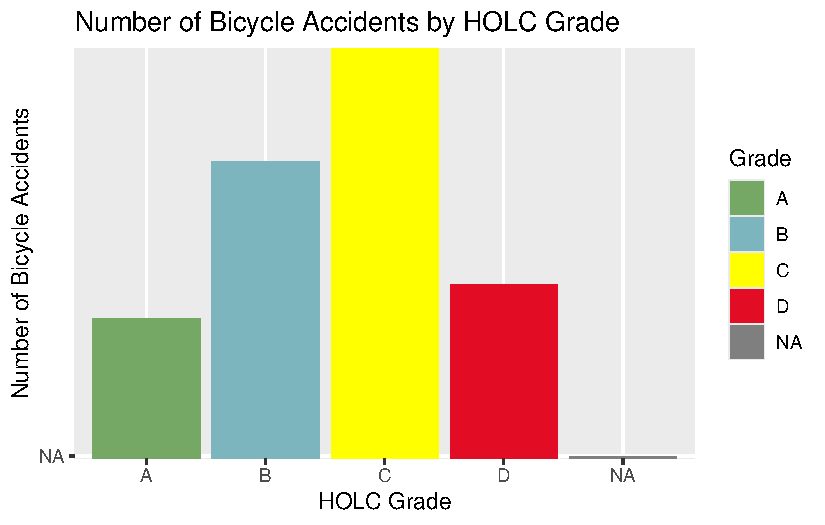
\includegraphics[keepaspectratio]{ejscreen_inequality_files/figure-pdf/unnamed-chunk-13-2.pdf}}

\begin{center}\rule{0.5\linewidth}{0.5pt}\end{center}




\end{document}
